\clearpage
\section{Targeted numerical replications}
\label{app:peer-review}

These extensions preserve the primary cohort and its grades. The numerical
objection replication changes the proposal policy and collection time while
holding source, author, frozen original and defence seed fixed. Literal
and automated source-audit grades remain separate; neither constitutes
independent human adjudication.

The rerun retains 1,500 assignments, 1,430 executed branches, 1,400 valid
defences and settled panels, and 30 aborted panels. Separate receipt checks
verify 14,118 confirmed transactions and 21,177 public event logs. Fresh
journals and spending ledgers preserve failures without replacement.
Of 300 originals, 286 scalar answers are eligible, 13 are unavailable and
one is unsupported.

\begin{figure}[htbp]
\centering
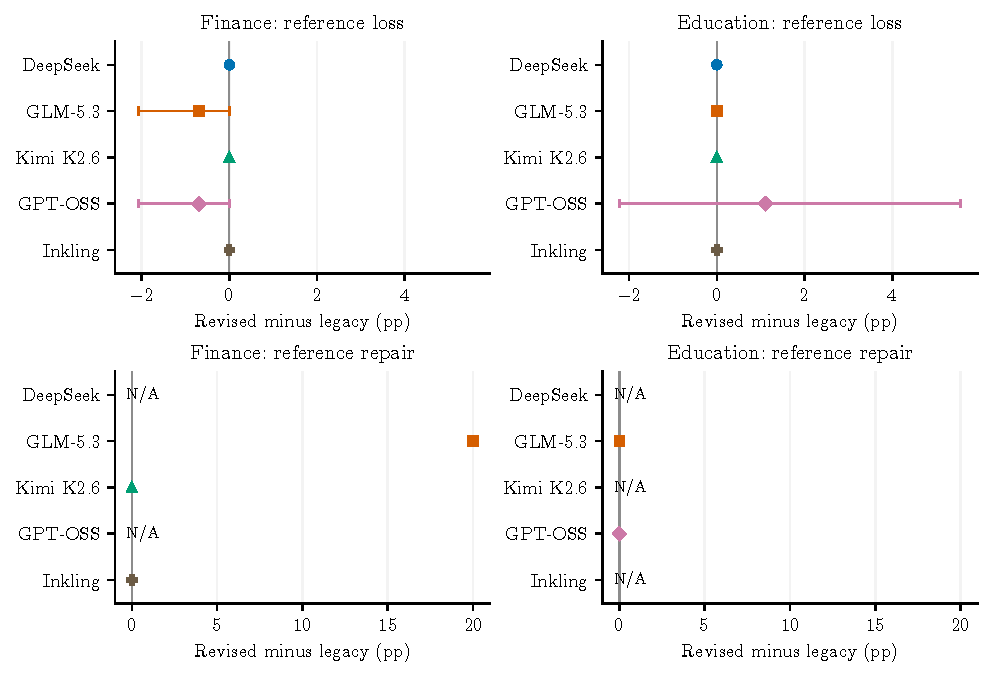
\includegraphics[width=\linewidth]{figures/peer-review-objection.pdf}
\caption{Paired change after the numerical objection-policy replacement,
under the automated source-audit sensitivity. Positive values indicate more
loss or repair with v2. Differences average matched seed outcomes within
source before 2,000 resamples in the original sampling strata. Whiskers are
pointwise 95\% percentile intervals. Missing paired outcomes are excluded
only from their corresponding contrast; no failed output is a wrong answer.
Single-source strata can yield collapsed intervals without population certainty.}
\label{fig:peer-review-objection}
\end{figure}

\begin{table}[htbp]
\centering\small\setlength{\tabcolsep}{3pt}
\begin{tabular}{llrrrrr}
\toprule
Model & Grade & Old loss & V2 loss & $\Delta$ loss, pp [95\% CI] & Old repair & V2 repair\\
\midrule
\input tables/peer-review-objection-rows.tex
\bottomrule
\end{tabular}
\caption{Paired eligible counts under literal and automated audited grades.
Loss is conditional on a matching original; repair is conditional on a
mismatching original. Each pair requires valid outcomes in both cohorts.
The interval describes the source-mean loss difference, v2 minus legacy;
the displayed counts pool eligible repeated outputs. Equal source weighting
can give a different direction from pooled counts when valid seed counts vary.
A zero denominator is
an unavailable comparison, not evidence of perfect behaviour.}
\label{tab:peer-review-objections}
\end{table}

\FloatBarrier
\subsection{Judge contexts and the historical trigger}
\label{app:peer-review-judges}

The false-claim cohort contains four operator-checked errors, including the
original GPN arithmetic trigger. The trigger-excluded comparison has only
three sources, including a one-source finance stratum. Its collapsed
within-stratum component cannot quantify uncertainty about unseen financial
cases. Correct controls are unchanged by trigger exclusion. These are
selected numerical cases and standalone judgments, not a prevalence sample
or additional Veracity settlements.

Three false defences are from GLM and one from Kimi; correct controls are from
DeepSeek (two), GPT-OSS (one) and Kimi (one). Controls match benchmarks,
not authors or difficulty. The ambiguous dandelion problem is withheld for
human review. The extension produces 681 valid judgments; DeepSeek accounts
for all 39 failures (37 output limits and two timeouts).

\begin{table}[htbp]
\centering\small\setlength{\tabcolsep}{3pt}
\begin{tabular}{lllrrrrr}
\toprule
Judge & Claim & Trigger & Claim only & Defended & Checked & $\Delta_D$, pp [95\% CI] & $\Delta_C$, pp [95\% CI]\\
\midrule
\input tables/peer-review-judge-rows.tex
\bottomrule
\end{tabular}
\caption{Correct judgments over valid outputs by context. $\Delta_D$ and
$\Delta_C$ compare defended and checked-evidence contexts with claim only,
respectively, using matched source/seed/call outcomes. Differences are
source means with pointwise 95\% source-group bootstrap intervals; counts
retain each condition's valid denominator. The checked context contains
both the defence and a correct calculation. Trigger exclusion changes only
the false-claim cohort.}
\label{tab:peer-review-judges}
\end{table}

\begin{table}[htbp]
\centering\small\setlength{\tabcolsep}{3pt}
\begin{tabular}{>{\raggedright\arraybackslash}p{.32\linewidth}llrrrr}
\toprule
Source task & Judge & Claim & Trigger & Claim only & Defended & Checked\\
\midrule
\input tables/peer-review-judge-cases-rows.tex
\bottomrule
\end{tabular}
\caption{All eight source groups by judge, showing correct/valid judgments
out of 15 assigned calls per context (five seeds, three repeated calls).
False denotes an operator-checked numerical error; True denotes a correct
control. The trigger column identifies the historical selected source.
Case-level readouts reveal whether an aggregate pattern recurs beyond it;
the calls within one source are not independent tasks.}
\label{tab:peer-review-judge-cases}
\end{table}
